% Options for packages loaded elsewhere
\PassOptionsToPackage{unicode}{hyperref}
\PassOptionsToPackage{hyphens}{url}
%
\documentclass[
  12pt,
]{article}
\usepackage{lmodern}
\usepackage{amssymb,amsmath}
\usepackage{ifxetex,ifluatex}
\ifnum 0\ifxetex 1\fi\ifluatex 1\fi=0 % if pdftex
  \usepackage[T1]{fontenc}
  \usepackage[utf8]{inputenc}
  \usepackage{textcomp} % provide euro and other symbols
\else % if luatex or xetex
  \usepackage{unicode-math}
  \defaultfontfeatures{Scale=MatchLowercase}
  \defaultfontfeatures[\rmfamily]{Ligatures=TeX,Scale=1}
  \setmainfont[]{Times New Roman}
\fi
% Use upquote if available, for straight quotes in verbatim environments
\IfFileExists{upquote.sty}{\usepackage{upquote}}{}
\IfFileExists{microtype.sty}{% use microtype if available
  \usepackage[]{microtype}
  \UseMicrotypeSet[protrusion]{basicmath} % disable protrusion for tt fonts
}{}
\makeatletter
\@ifundefined{KOMAClassName}{% if non-KOMA class
  \IfFileExists{parskip.sty}{%
    \usepackage{parskip}
  }{% else
    \setlength{\parindent}{0pt}
    \setlength{\parskip}{6pt plus 2pt minus 1pt}}
}{% if KOMA class
  \KOMAoptions{parskip=half}}
\makeatother
\usepackage{xcolor}
\IfFileExists{xurl.sty}{\usepackage{xurl}}{} % add URL line breaks if available
\IfFileExists{bookmark.sty}{\usepackage{bookmark}}{\usepackage{hyperref}}
\hypersetup{
  pdftitle={Comparison of community and citizen natural resource rights across Sub-Saharan Africa},
  pdfauthor={Kim Myers},
  hidelinks,
  pdfcreator={LaTeX via pandoc}}
\urlstyle{same} % disable monospaced font for URLs
\usepackage[margin=2.54cm]{geometry}
\usepackage{color}
\usepackage{fancyvrb}
\newcommand{\VerbBar}{|}
\newcommand{\VERB}{\Verb[commandchars=\\\{\}]}
\DefineVerbatimEnvironment{Highlighting}{Verbatim}{commandchars=\\\{\}}
% Add ',fontsize=\small' for more characters per line
\usepackage{framed}
\definecolor{shadecolor}{RGB}{248,248,248}
\newenvironment{Shaded}{\begin{snugshade}}{\end{snugshade}}
\newcommand{\AlertTok}[1]{\textcolor[rgb]{0.94,0.16,0.16}{#1}}
\newcommand{\AnnotationTok}[1]{\textcolor[rgb]{0.56,0.35,0.01}{\textbf{\textit{#1}}}}
\newcommand{\AttributeTok}[1]{\textcolor[rgb]{0.77,0.63,0.00}{#1}}
\newcommand{\BaseNTok}[1]{\textcolor[rgb]{0.00,0.00,0.81}{#1}}
\newcommand{\BuiltInTok}[1]{#1}
\newcommand{\CharTok}[1]{\textcolor[rgb]{0.31,0.60,0.02}{#1}}
\newcommand{\CommentTok}[1]{\textcolor[rgb]{0.56,0.35,0.01}{\textit{#1}}}
\newcommand{\CommentVarTok}[1]{\textcolor[rgb]{0.56,0.35,0.01}{\textbf{\textit{#1}}}}
\newcommand{\ConstantTok}[1]{\textcolor[rgb]{0.00,0.00,0.00}{#1}}
\newcommand{\ControlFlowTok}[1]{\textcolor[rgb]{0.13,0.29,0.53}{\textbf{#1}}}
\newcommand{\DataTypeTok}[1]{\textcolor[rgb]{0.13,0.29,0.53}{#1}}
\newcommand{\DecValTok}[1]{\textcolor[rgb]{0.00,0.00,0.81}{#1}}
\newcommand{\DocumentationTok}[1]{\textcolor[rgb]{0.56,0.35,0.01}{\textbf{\textit{#1}}}}
\newcommand{\ErrorTok}[1]{\textcolor[rgb]{0.64,0.00,0.00}{\textbf{#1}}}
\newcommand{\ExtensionTok}[1]{#1}
\newcommand{\FloatTok}[1]{\textcolor[rgb]{0.00,0.00,0.81}{#1}}
\newcommand{\FunctionTok}[1]{\textcolor[rgb]{0.00,0.00,0.00}{#1}}
\newcommand{\ImportTok}[1]{#1}
\newcommand{\InformationTok}[1]{\textcolor[rgb]{0.56,0.35,0.01}{\textbf{\textit{#1}}}}
\newcommand{\KeywordTok}[1]{\textcolor[rgb]{0.13,0.29,0.53}{\textbf{#1}}}
\newcommand{\NormalTok}[1]{#1}
\newcommand{\OperatorTok}[1]{\textcolor[rgb]{0.81,0.36,0.00}{\textbf{#1}}}
\newcommand{\OtherTok}[1]{\textcolor[rgb]{0.56,0.35,0.01}{#1}}
\newcommand{\PreprocessorTok}[1]{\textcolor[rgb]{0.56,0.35,0.01}{\textit{#1}}}
\newcommand{\RegionMarkerTok}[1]{#1}
\newcommand{\SpecialCharTok}[1]{\textcolor[rgb]{0.00,0.00,0.00}{#1}}
\newcommand{\SpecialStringTok}[1]{\textcolor[rgb]{0.31,0.60,0.02}{#1}}
\newcommand{\StringTok}[1]{\textcolor[rgb]{0.31,0.60,0.02}{#1}}
\newcommand{\VariableTok}[1]{\textcolor[rgb]{0.00,0.00,0.00}{#1}}
\newcommand{\VerbatimStringTok}[1]{\textcolor[rgb]{0.31,0.60,0.02}{#1}}
\newcommand{\WarningTok}[1]{\textcolor[rgb]{0.56,0.35,0.01}{\textbf{\textit{#1}}}}
\usepackage{graphicx,grffile}
\makeatletter
\def\maxwidth{\ifdim\Gin@nat@width>\linewidth\linewidth\else\Gin@nat@width\fi}
\def\maxheight{\ifdim\Gin@nat@height>\textheight\textheight\else\Gin@nat@height\fi}
\makeatother
% Scale images if necessary, so that they will not overflow the page
% margins by default, and it is still possible to overwrite the defaults
% using explicit options in \includegraphics[width, height, ...]{}
\setkeys{Gin}{width=\maxwidth,height=\maxheight,keepaspectratio}
% Set default figure placement to htbp
\makeatletter
\def\fps@figure{htbp}
\makeatother
\setlength{\emergencystretch}{3em} % prevent overfull lines
\providecommand{\tightlist}{%
  \setlength{\itemsep}{0pt}\setlength{\parskip}{0pt}}
\setcounter{secnumdepth}{5}
\usepackage{booktabs}
\usepackage{longtable}
\usepackage{array}
\usepackage{multirow}
\usepackage{wrapfig}
\usepackage{float}
\usepackage{colortbl}
\usepackage{pdflscape}
\usepackage{tabu}
\usepackage{threeparttable}
\usepackage{threeparttablex}
\usepackage[normalem]{ulem}
\usepackage{makecell}
\usepackage{xcolor}

\title{Comparison of community and citizen natural resource rights across
Sub-Saharan Africa}
\usepackage{etoolbox}
\makeatletter
\providecommand{\subtitle}[1]{% add subtitle to \maketitle
  \apptocmd{\@title}{\par {\large #1 \par}}{}{}
}
\makeatother
\subtitle{\url{https://github.com/krm75/Environmental_Data_Analytics_2020/tree/master/ResourceRights}}
\author{Kim Myers}
\date{}

\begin{document}
\maketitle

\newpage
\tableofcontents 
\newpage
\listoftables 
\newpage
\listoffigures 
\newpage

\hypertarget{rationale-and-research-questions}{%
\section{Rationale and Research
Questions}\label{rationale-and-research-questions}}

\newpage

\hypertarget{dataset-information}{%
\section{Dataset Information}\label{dataset-information}}

\begin{Shaded}
\begin{Highlighting}[]
\KeywordTok{kable}\NormalTok{(}\KeywordTok{head}\NormalTok{(wildlife),}
\DataTypeTok{caption =} \StringTok{"Table 1: First 10 rows of the 5 raw data sets, 1 for each resource."}\NormalTok{) }\OperatorTok
\StringTok{  }\KeywordTok{kable_styling}\NormalTok{(}\DataTypeTok{bootstrap_options =} \KeywordTok{c}\NormalTok{(}\StringTok{"hover"}\NormalTok{, }\StringTok{"condensed"}\NormalTok{),}\DataTypeTok{full_width =}\NormalTok{ F) }\OperatorTok
\StringTok{  }\KeywordTok{column_spec}\NormalTok{(}\DecValTok{3}\OperatorTok{:}\DecValTok{13}\NormalTok{, }\DataTypeTok{width_min =} \StringTok{"4em"}\NormalTok{, }\DataTypeTok{width_max =} \StringTok{"4em"}\NormalTok{)}
\end{Highlighting}
\end{Shaded}

\begin{table}

\caption{\label{tab:unnamed-chunk-1}Table 1: First 10 rows of the 5 raw data sets, 1 for each resource.}
\centering
\begin{tabular}[t]{l|l|>{}l|>{}l|>{}l|>{}l|>{}l|>{}l|>{}l|>{}l|>{}l|>{}l|>{}l}
\hline
Country.code & Country & Q1 & Q2 & Q3 & Q4 & Q5 & Q6 & Q7 & Q8 & Q9 & Q10 & Q11\\
\hline
AO & Angola & Yes, implied & No & Yes & Yes & Partial & Partial & No & Yes & Partial & Yes, implied & No\\
\hline
BN & Benin & Yes & No & Yes & Yes & Yes & No & No & Yes & Partial & Yes, implied & No\\
\hline
BC & Botswana & Yes, implied & Yes & Silent & Yes & Partial & No & No & Yes & Yes & Yes & Yes, implied\\
\hline
UV & Burkina Faso & Yes, implied & No, implied & Yes & No & No & No & No & No & No & No & No\\
\hline
BY & Burundi & Yes, implied & No, implied & Silent & Yes & No & No & No & Yes & No & No & No\\
\hline
CM & Cameroon & Yes, implied & No, implied & Yes & Yes & No & No & Silent & Yes & Partial & Yes, implied & No\\
\hline
\end{tabular}
\end{table}

\newpage

\hypertarget{exploratory-analysis-and-data-wrangling}{%
\section{Exploratory Analysis and Data
Wrangling}\label{exploratory-analysis-and-data-wrangling}}

\begin{Shaded}
\begin{Highlighting}[]
\KeywordTok{length}\NormalTok{(}\KeywordTok{unique}\NormalTok{(wildlife}\OperatorTok{$}\NormalTok{Country))}
\end{Highlighting}
\end{Shaded}

\begin{verbatim}
## [1] 49
\end{verbatim}

\begin{Shaded}
\begin{Highlighting}[]
\KeywordTok{unique}\NormalTok{(wildlife}\OperatorTok{$}\NormalTok{Country)}
\end{Highlighting}
\end{Shaded}

\begin{verbatim}
##  [1] Angola                          Benin                          
##  [3] Botswana                        Burkina Faso                   
##  [5] Burundi                         Cameroon                       
##  [7] Cape Verde                      Central African Republic       
##  [9] Chad                            Comoros                        
## [11] Cote d'Ivoire                   Djibouti                       
## [13] Democratic Republic of Congo    Equatorial Guinea              
## [15] Eritrea                         Ethiopia                       
## [17] Gabon                           Gambia                         
## [19] Ghana                           Guinea                         
## [21] Guinea-Bissau                   Kenya                          
## [23] Lesotho                         Liberia                        
## [25] Madagascar                      Malawi                         
## [27] Mali                            Mauritania                     
## [29] Mauritius                       Mozambique                     
## [31] Namibia                         Niger                          
## [33] Nigeria                         Republic of Congo (Brazzaville)
## [35] Rwanda                          Sao Tome and Principe          
## [37] Senegal                         Seychelles                     
## [39] Sierra Leone                    Somalia                        
## [41] South Africa                    South Sudan                    
## [43] Sudan                           Swaziland                      
## [45] Tanzania                        Togo                           
## [47] Uganda                          Zambia                         
## [49] Zimbabwe                       
## 49 Levels: Angola Benin Botswana Burkina Faso Burundi Cameroon ... Zimbabwe
\end{verbatim}

\begin{Shaded}
\begin{Highlighting}[]
\KeywordTok{nrow}\NormalTok{(wildlife)}
\end{Highlighting}
\end{Shaded}

\begin{verbatim}
## [1] 49
\end{verbatim}

\begin{Shaded}
\begin{Highlighting}[]
\KeywordTok{ncol}\NormalTok{(wildlife)}
\end{Highlighting}
\end{Shaded}

\begin{verbatim}
## [1] 13
\end{verbatim}

\begin{Shaded}
\begin{Highlighting}[]
\KeywordTok{colnames}\NormalTok{(wildlife)}
\end{Highlighting}
\end{Shaded}

\begin{verbatim}
##  [1] "Country.code" "Country"      "Q1"           "Q2"           "Q3"          
##  [6] "Q4"           "Q5"           "Q6"           "Q7"           "Q8"          
## [11] "Q9"           "Q10"          "Q11"
\end{verbatim}

\begin{Shaded}
\begin{Highlighting}[]
\KeywordTok{str}\NormalTok{(wildlife)}
\end{Highlighting}
\end{Shaded}

\begin{verbatim}
## 'data.frame':    49 obs. of  13 variables:
##  $ Country.code: Factor w/ 49 levels "AO","BC","BN",..: 1 3 2 45 4 8 11 10 5 9 ...
##  $ Country     : Factor w/ 49 levels "Angola","Benin",..: 1 2 3 4 5 6 7 8 9 10 ...
##  $ Q1          : Factor w/ 4 levels "No information available",..: 4 3 4 4 4 4 2 3 4 1 ...
##  $ Q2          : Factor w/ 6 levels "No","No information available",..: 1 1 5 3 3 3 4 1 4 2 ...
##  $ Q3          : Factor w/ 4 levels "No information available",..: 3 3 2 3 2 3 2 3 3 1 ...
##  $ Q4          : Factor w/ 6 levels "No","No information available",..: 5 5 5 1 5 5 1 5 5 2 ...
##  $ Q5          : Factor w/ 6 levels "No","No information available",..: 3 5 3 1 1 1 1 3 3 2 ...
##  $ Q6          : Factor w/ 5 levels "No","No information available",..: 4 1 1 1 1 1 1 1 5 2 ...
##  $ Q7          : Factor w/ 6 levels "No","No information available",..: 1 1 1 1 1 4 1 3 4 2 ...
##  $ Q8          : Factor w/ 5 levels "No","No information available",..: 4 4 4 1 4 4 1 4 4 2 ...
##  $ Q9          : Factor w/ 6 levels "No","No information available",..: 3 3 5 1 1 3 1 3 3 2 ...
##  $ Q10         : Factor w/ 6 levels "No","No information available",..: 6 6 5 1 1 6 1 3 1 2 ...
##  $ Q11         : Factor w/ 5 levels "No","No information available",..: 1 1 5 1 1 1 1 1 1 2 ...
\end{verbatim}

\begin{Shaded}
\begin{Highlighting}[]
\CommentTok{#summary(wildlife)}
\NormalTok{yes <-}\StringTok{ }\KeywordTok{c}\NormalTok{(}\StringTok{'Yes'}\NormalTok{,}\StringTok{'Yes, implied'}\NormalTok{)}
\NormalTok{no <-}\StringTok{ }\KeywordTok{c}\NormalTok{(}\StringTok{'No'}\NormalTok{,}\StringTok{'No information available'}\NormalTok{,}\StringTok{'No, implied'}\NormalTok{,}\StringTok{'Silent'}\NormalTok{)}


\NormalTok{wildlife[,}\KeywordTok{c}\NormalTok{(}\DecValTok{4}\OperatorTok{:}\DecValTok{6}\NormalTok{,}\DecValTok{8}\OperatorTok{:}\DecValTok{9}\NormalTok{,}\DecValTok{11}\NormalTok{,}\DecValTok{13}\NormalTok{)] <-}\StringTok{ }\KeywordTok{sapply}\NormalTok{(wildlife[,}\KeywordTok{c}\NormalTok{(}\DecValTok{4}\OperatorTok{:}\DecValTok{6}\NormalTok{,}\DecValTok{8}\OperatorTok{:}\DecValTok{9}\NormalTok{,}\DecValTok{11}\NormalTok{,}\DecValTok{13}\NormalTok{)], }\DataTypeTok{FUN =} \ControlFlowTok{function}\NormalTok{(x) }\KeywordTok{ifelse}\NormalTok{(x }\OperatorTok\StringTok{ }\NormalTok{yes, }\DecValTok{1}\NormalTok{, }\DecValTok{0}\NormalTok{))}
\NormalTok{wildlife}\OperatorTok{$}\NormalTok{count <-}\StringTok{ }\KeywordTok{apply}\NormalTok{(wildlife[,}\KeywordTok{c}\NormalTok{(}\DecValTok{4}\OperatorTok{:}\DecValTok{6}\NormalTok{,}\DecValTok{8}\OperatorTok{:}\DecValTok{9}\NormalTok{,}\DecValTok{11}\NormalTok{,}\DecValTok{13}\NormalTok{)],}\DecValTok{1}\NormalTok{,sum)}

\NormalTok{minerals[,}\KeywordTok{c}\NormalTok{(}\DecValTok{4}\OperatorTok{:}\DecValTok{6}\NormalTok{,}\DecValTok{8}\OperatorTok{:}\DecValTok{9}\NormalTok{,}\DecValTok{11}\NormalTok{,}\DecValTok{13}\NormalTok{)] <-}\StringTok{ }\KeywordTok{sapply}\NormalTok{(minerals[,}\KeywordTok{c}\NormalTok{(}\DecValTok{4}\OperatorTok{:}\DecValTok{6}\NormalTok{,}\DecValTok{8}\OperatorTok{:}\DecValTok{9}\NormalTok{,}\DecValTok{11}\NormalTok{,}\DecValTok{13}\NormalTok{)], }\DataTypeTok{FUN =} \ControlFlowTok{function}\NormalTok{(x) }\KeywordTok{ifelse}\NormalTok{(x }\OperatorTok\StringTok{ }\NormalTok{yes, }\DecValTok{1}\NormalTok{, }\DecValTok{0}\NormalTok{))}
\NormalTok{minerals}\OperatorTok{$}\NormalTok{count <-}\StringTok{ }\KeywordTok{apply}\NormalTok{(minerals[,}\KeywordTok{c}\NormalTok{(}\DecValTok{4}\OperatorTok{:}\DecValTok{6}\NormalTok{,}\DecValTok{8}\OperatorTok{:}\DecValTok{9}\NormalTok{,}\DecValTok{11}\NormalTok{,}\DecValTok{13}\NormalTok{)],}\DecValTok{1}\NormalTok{,sum)}

\NormalTok{water[,}\KeywordTok{c}\NormalTok{(}\DecValTok{4}\OperatorTok{:}\DecValTok{6}\NormalTok{,}\DecValTok{8}\OperatorTok{:}\DecValTok{9}\NormalTok{,}\DecValTok{11}\NormalTok{,}\DecValTok{13}\NormalTok{)] <-}\StringTok{ }\KeywordTok{sapply}\NormalTok{(water[,}\KeywordTok{c}\NormalTok{(}\DecValTok{4}\OperatorTok{:}\DecValTok{6}\NormalTok{,}\DecValTok{8}\OperatorTok{:}\DecValTok{9}\NormalTok{,}\DecValTok{11}\NormalTok{,}\DecValTok{13}\NormalTok{)], }\DataTypeTok{FUN =} \ControlFlowTok{function}\NormalTok{(x) }\KeywordTok{ifelse}\NormalTok{(x }\OperatorTok\StringTok{ }\NormalTok{yes, }\DecValTok{1}\NormalTok{, }\DecValTok{0}\NormalTok{))}
\NormalTok{water}\OperatorTok{$}\NormalTok{count <-}\StringTok{ }\KeywordTok{apply}\NormalTok{(water[,}\KeywordTok{c}\NormalTok{(}\DecValTok{4}\OperatorTok{:}\DecValTok{6}\NormalTok{,}\DecValTok{8}\OperatorTok{:}\DecValTok{9}\NormalTok{,}\DecValTok{11}\NormalTok{,}\DecValTok{13}\NormalTok{)],}\DecValTok{1}\NormalTok{,sum)}

\NormalTok{petroleum[,}\KeywordTok{c}\NormalTok{(}\DecValTok{4}\OperatorTok{:}\DecValTok{6}\NormalTok{,}\DecValTok{8}\OperatorTok{:}\DecValTok{9}\NormalTok{,}\DecValTok{11}\NormalTok{,}\DecValTok{13}\NormalTok{)] <-}\StringTok{ }\KeywordTok{sapply}\NormalTok{(petroleum[,}\KeywordTok{c}\NormalTok{(}\DecValTok{4}\OperatorTok{:}\DecValTok{6}\NormalTok{,}\DecValTok{8}\OperatorTok{:}\DecValTok{9}\NormalTok{,}\DecValTok{11}\NormalTok{,}\DecValTok{13}\NormalTok{)], }\DataTypeTok{FUN =} \ControlFlowTok{function}\NormalTok{(x) }\KeywordTok{ifelse}\NormalTok{(x }\OperatorTok\StringTok{ }\NormalTok{yes, }\DecValTok{1}\NormalTok{, }\DecValTok{0}\NormalTok{))}
\NormalTok{petroleum}\OperatorTok{$}\NormalTok{count <-}\StringTok{ }\KeywordTok{apply}\NormalTok{(petroleum[,}\KeywordTok{c}\NormalTok{(}\DecValTok{4}\OperatorTok{:}\DecValTok{6}\NormalTok{,}\DecValTok{8}\OperatorTok{:}\DecValTok{9}\NormalTok{,}\DecValTok{11}\NormalTok{,}\DecValTok{13}\NormalTok{)],}\DecValTok{1}\NormalTok{,sum)}

\NormalTok{trees[,}\KeywordTok{c}\NormalTok{(}\DecValTok{4}\OperatorTok{:}\DecValTok{6}\NormalTok{,}\DecValTok{8}\OperatorTok{:}\DecValTok{9}\NormalTok{,}\DecValTok{11}\NormalTok{,}\DecValTok{13}\NormalTok{)] <-}\StringTok{ }\KeywordTok{sapply}\NormalTok{(trees[,}\KeywordTok{c}\NormalTok{(}\DecValTok{4}\OperatorTok{:}\DecValTok{6}\NormalTok{,}\DecValTok{8}\OperatorTok{:}\DecValTok{9}\NormalTok{,}\DecValTok{11}\NormalTok{,}\DecValTok{13}\NormalTok{)], }\DataTypeTok{FUN =} \ControlFlowTok{function}\NormalTok{(x) }\KeywordTok{ifelse}\NormalTok{(x }\OperatorTok\StringTok{ }\NormalTok{yes, }\DecValTok{1}\NormalTok{, }\DecValTok{0}\NormalTok{))}
\NormalTok{trees}\OperatorTok{$}\NormalTok{count <-}\StringTok{ }\KeywordTok{apply}\NormalTok{(trees[,}\KeywordTok{c}\NormalTok{(}\DecValTok{4}\OperatorTok{:}\DecValTok{6}\NormalTok{,}\DecValTok{8}\OperatorTok{:}\DecValTok{9}\NormalTok{,}\DecValTok{11}\NormalTok{,}\DecValTok{13}\NormalTok{)],}\DecValTok{1}\NormalTok{,sum)}


\NormalTok{countrycounts <-}\StringTok{ }\KeywordTok{data.frame}\NormalTok{(wildlife}\OperatorTok{$}\NormalTok{Country,wildlife}\OperatorTok{$}\NormalTok{count,minerals}\OperatorTok{$}\NormalTok{count,water}\OperatorTok{$}\NormalTok{count,petroleum}\OperatorTok{$}\NormalTok{count,trees}\OperatorTok{$}\NormalTok{count)}
\NormalTok{countrycounts}\OperatorTok{$}\NormalTok{Total <-}\StringTok{ }\KeywordTok{apply}\NormalTok{(countrycounts[,}\KeywordTok{c}\NormalTok{(}\DecValTok{2}\OperatorTok{:}\DecValTok{6}\NormalTok{)],}\DecValTok{1}\NormalTok{,sum)}\OperatorTok{/}\DecValTok{35}
\KeywordTok{colnames}\NormalTok{(countrycounts) <-}\StringTok{ }\KeywordTok{c}\NormalTok{(}\StringTok{"Country"}\NormalTok{,}\StringTok{"Wildlife"}\NormalTok{,}\StringTok{"Minerals"}\NormalTok{,}\StringTok{"Water"}\NormalTok{,}\StringTok{"Petroleum"}\NormalTok{,}\StringTok{"Trees"}\NormalTok{,}\StringTok{"Total"}\NormalTok{)}

\KeywordTok{kable}\NormalTok{(countrycounts[}\KeywordTok{order}\NormalTok{(}\OperatorTok{-}\NormalTok{countrycounts}\OperatorTok{$}\NormalTok{Total),],}
\DataTypeTok{caption =} \StringTok{"Table 2: Number of survey question responses that support individual/community resource rights to some degree."}\NormalTok{, }\DataTypeTok{row.names =}\NormalTok{ F)  }\OperatorTok
\StringTok{  }\KeywordTok{kable_styling}\NormalTok{(}\DataTypeTok{bootstrap_options =} \KeywordTok{c}\NormalTok{(}\StringTok{"hover"}\NormalTok{, }\StringTok{"condensed"}\NormalTok{),}\DataTypeTok{full_width =}\NormalTok{ F) }\CommentTok{#%>%}
\end{Highlighting}
\end{Shaded}

\begin{table}

\caption{\label{tab:unnamed-chunk-8}Table 2: Number of survey question responses that support individual/community resource rights to some degree.}
\centering
\begin{tabular}[t]{l|r|r|r|r|r|r}
\hline
Country & Wildlife & Minerals & Water & Petroleum & Trees & Total\\
\hline
Botswana & 4 & 4 & 4 & 0 & 4 & 0.4571429\\
\hline
Namibia & 6 & 2 & 4 & 0 & 4 & 0.4571429\\
\hline
Tanzania & 2 & 3 & 3 & 0 & 5 & 0.3714286\\
\hline
Central African Republic & 2 & 0 & 5 & 0 & 5 & 0.3428571\\
\hline
Mali & 2 & 4 & 3 & 0 & 2 & 0.3142857\\
\hline
South Africa & 3 & 2 & 3 & 0 & 3 & 0.3142857\\
\hline
Cameroon & 2 & 1 & 3 & 0 & 4 & 0.2857143\\
\hline
Gambia & 1 & 0 & 4 & 0 & 5 & 0.2857143\\
\hline
Guinea & 3 & 1 & 3 & 0 & 3 & 0.2857143\\
\hline
Mozambique & 3 & 1 & 4 & 0 & 2 & 0.2857143\\
\hline
Somalia & 3 & 0 & 3 & 0 & 4 & 0.2857143\\
\hline
Angola & 2 & 0 & 4 & 0 & 3 & 0.2571429\\
\hline
Benin & 2 & 0 & 5 & 0 & 2 & 0.2571429\\
\hline
Burkina Faso & 1 & 2 & 3 & 0 & 3 & 0.2571429\\
\hline
Cote d'Ivoire & 2 & 0 & 4 & 0 & 3 & 0.2571429\\
\hline
Ethiopia & 2 & 2 & 4 & 0 & 1 & 0.2571429\\
\hline
Malawi & 3 & 0 & 3 & 0 & 3 & 0.2571429\\
\hline
Mauritius & 2 & 2 & 3 & 0 & 2 & 0.2571429\\
\hline
Republic of Congo (Brazzaville) & 2 & 2 & 3 & 0 & 2 & 0.2571429\\
\hline
Togo & 3 & 0 & 3 & 0 & 3 & 0.2571429\\
\hline
Zimbabwe & 1 & 1 & 4 & 0 & 3 & 0.2571429\\
\hline
Chad & 2 & 0 & 3 & 0 & 3 & 0.2285714\\
\hline
Ghana & 1 & 2 & 3 & 0 & 2 & 0.2285714\\
\hline
Kenya & 1 & 1 & 2 & 0 & 4 & 0.2285714\\
\hline
Niger & 2 & 1 & 2 & 0 & 3 & 0.2285714\\
\hline
Nigeria & 3 & 1 & 1 & 0 & 3 & 0.2285714\\
\hline
Sierra Leone & 1 & 0 & 4 & 0 & 3 & 0.2285714\\
\hline
Zambia & 2 & 0 & 3 & 0 & 3 & 0.2285714\\
\hline
Gabon & 3 & 2 & 0 & 0 & 2 & 0.2000000\\
\hline
Lesotho & 1 & 3 & 2 & 0 & 1 & 0.2000000\\
\hline
Madagascar & 1 & 0 & 3 & 0 & 3 & 0.2000000\\
\hline
South Sudan & 3 & 0 & 2 & 0 & 2 & 0.2000000\\
\hline
Sudan & 3 & 2 & 0 & 0 & 2 & 0.2000000\\
\hline
Swaziland & 2 & 0 & 3 & 0 & 2 & 0.2000000\\
\hline
Uganda & 2 & 1 & 1 & 0 & 3 & 0.2000000\\
\hline
Guinea-Bissau & 2 & 0 & 2 & 0 & 2 & 0.1714286\\
\hline
Liberia & 2 & 0 & 1 & 0 & 3 & 0.1714286\\
\hline
Senegal & 3 & 0 & 1 & 0 & 2 & 0.1714286\\
\hline
Burundi & 1 & 1 & 1 & 0 & 2 & 0.1428571\\
\hline
Djibouti & 0 & 0 & 1 & 0 & 4 & 0.1428571\\
\hline
Eritrea & 0 & 0 & 3 & 0 & 2 & 0.1428571\\
\hline
Rwanda & 1 & 0 & 2 & 0 & 2 & 0.1428571\\
\hline
Comoros & 0 & 0 & 1 & 0 & 3 & 0.1142857\\
\hline
Democratic Republic of Congo & 2 & 0 & 2 & 0 & 0 & 0.1142857\\
\hline
Equatorial Guinea & 0 & 1 & 0 & 0 & 3 & 0.1142857\\
\hline
Mauritania & 1 & 0 & 1 & 0 & 2 & 0.1142857\\
\hline
Cape Verde & 0 & 0 & 1 & 0 & 1 & 0.0571429\\
\hline
Sao Tome and Principe & 0 & 0 & 0 & 0 & 1 & 0.0285714\\
\hline
Seychelles & 0 & 0 & 1 & 0 & 0 & 0.0285714\\
\hline
\end{tabular}
\end{table}

\begin{Shaded}
\begin{Highlighting}[]
  \CommentTok{#column_spec(3:13, width_min = "4em", width_max = "4em")}
\end{Highlighting}
\end{Shaded}

\begin{figure}
\centering
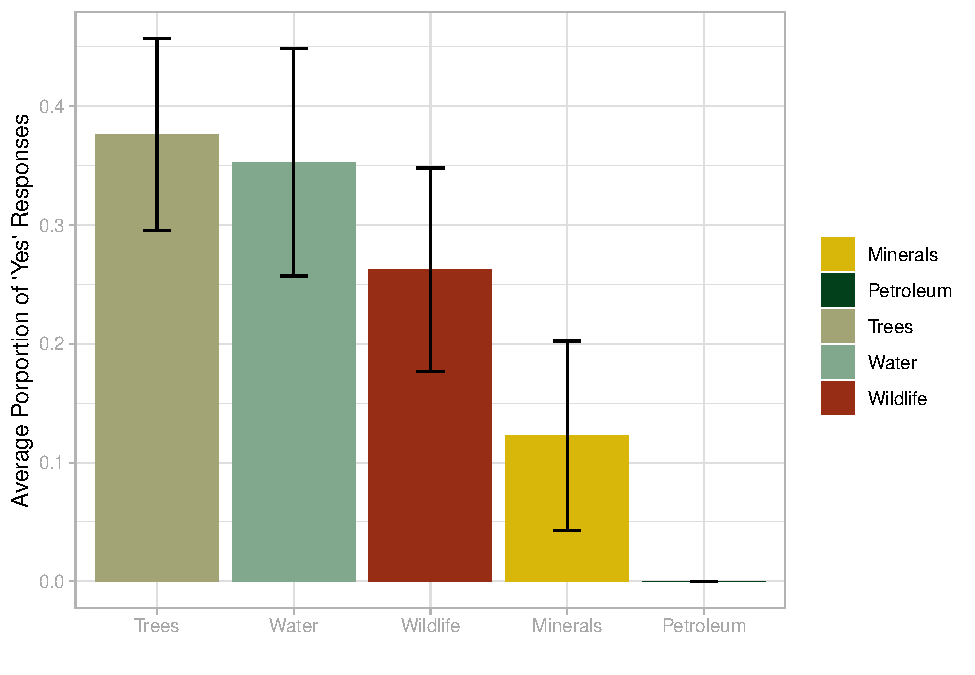
\includegraphics{FinalProject_Myers_files/figure-latex/fig1-1.pdf}
\caption{Average proportion of survey responses which support
individual/community resource rights to some degree by resource type.}
\end{figure}

\newpage

\hypertarget{analysis}{%
\section{Analysis}\label{analysis}}

\begin{figure}
\centering
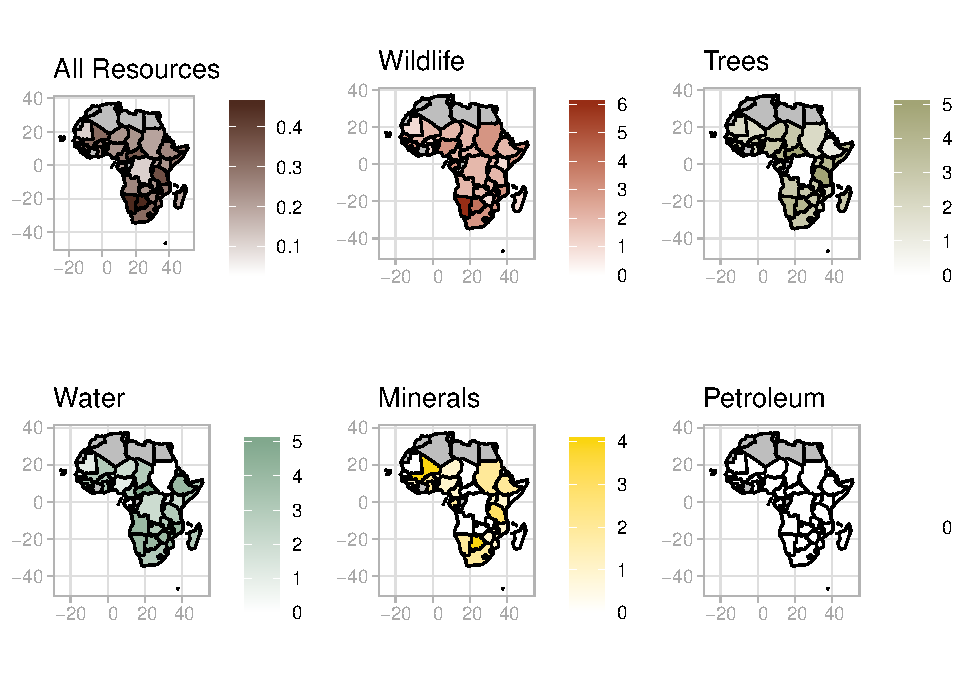
\includegraphics{FinalProject_Myers_files/figure-latex/unnamed-chunk-9-1.pdf}
\caption{Total number of survey questions from the Rights to Resources
dataset that support individual or community resource rights. The
highest possible sum for each resource was 7. In the All Resources
panel, values equal the proportion of responses that promote resource
rights.}
\end{figure}

\begin{Shaded}
\begin{Highlighting}[]
\NormalTok{country.counts.rcorr <-}\StringTok{ }\KeywordTok{cor}\NormalTok{(countrycounts[,}\KeywordTok{c}\NormalTok{(}\DecValTok{2}\OperatorTok{:}\DecValTok{4}\NormalTok{,}\DecValTok{6}\NormalTok{)])}

\KeywordTok{corrplot}\NormalTok{(country.counts.rcorr) }\CommentTok{#discluded petroleum}
\end{Highlighting}
\end{Shaded}

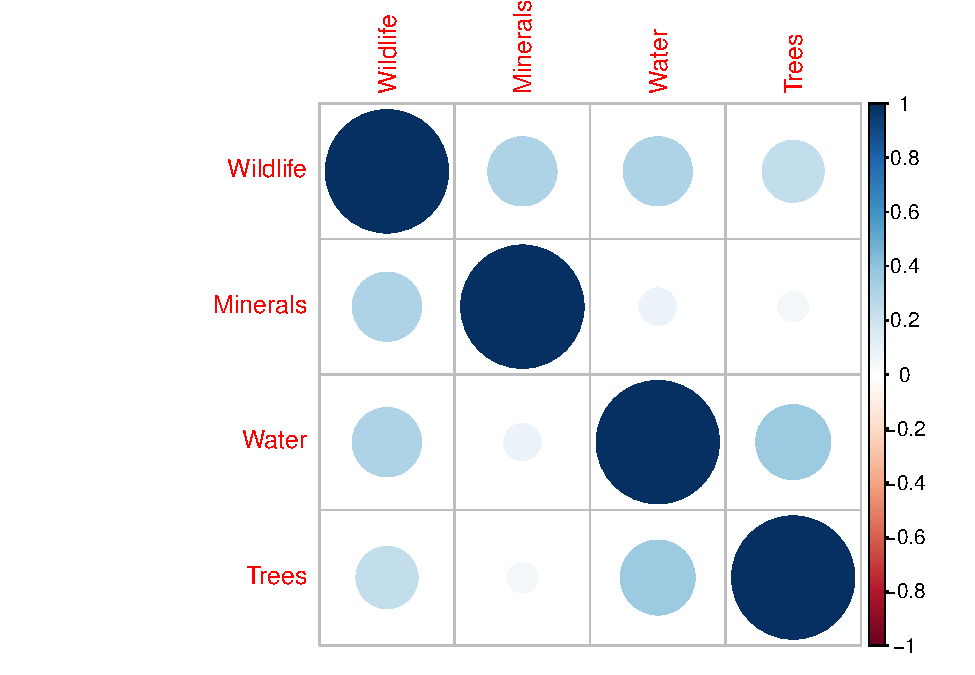
\includegraphics{FinalProject_Myers_files/figure-latex/unnamed-chunk-10-1.pdf}

\begin{Shaded}
\begin{Highlighting}[]
\KeywordTok{ggplot}\NormalTok{(countrycounts) }\OperatorTok{+}
\StringTok{  }\KeywordTok{geom_point}\NormalTok{(}\KeywordTok{aes}\NormalTok{(}\DataTypeTok{x=}\NormalTok{Wildlife, }\DataTypeTok{y=}\NormalTok{Minerals)) }\OperatorTok{+}
\StringTok{  }\KeywordTok{geom_point}\NormalTok{(}\KeywordTok{aes}\NormalTok{(}\DataTypeTok{x=}\NormalTok{Wildlife, }\DataTypeTok{y=}\NormalTok{Water)) }\OperatorTok{+}
\StringTok{  }\KeywordTok{geom_point}\NormalTok{(}\KeywordTok{aes}\NormalTok{(}\DataTypeTok{x=}\NormalTok{Wildlife, }\DataTypeTok{y=}\NormalTok{Trees))}
\end{Highlighting}
\end{Shaded}

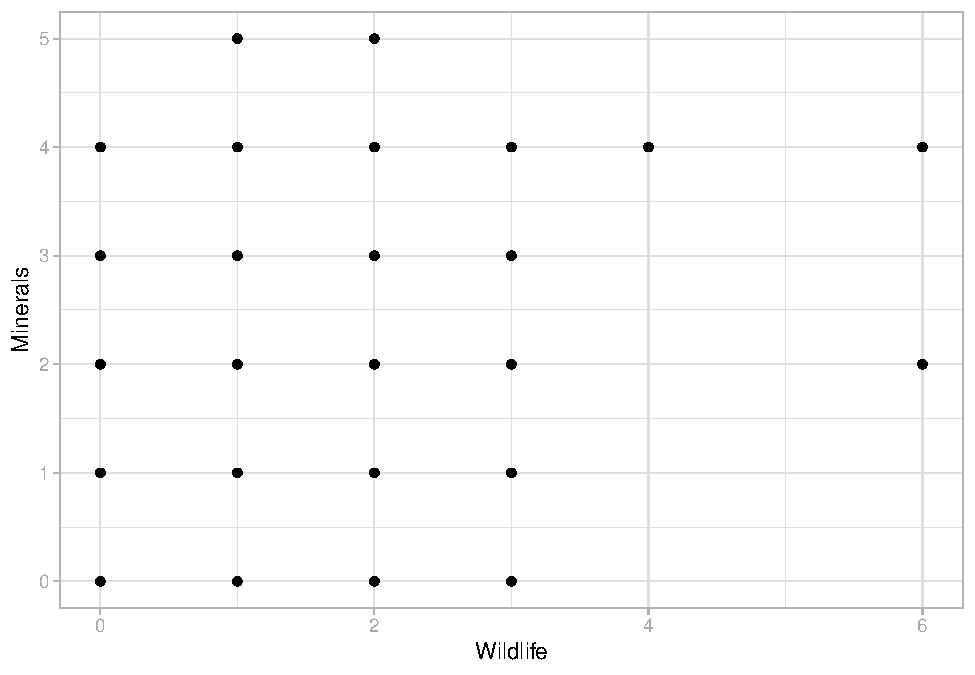
\includegraphics{FinalProject_Myers_files/figure-latex/unnamed-chunk-11-1.pdf}

\hypertarget{question-1-insert-specific-question-here-and-add-additional-subsections-for-additional-questions-below-if-needed}{%
\subsection{Question 1: \textless insert specific question here and add
additional subsections for additional questions below, if
needed\textgreater{}}\label{question-1-insert-specific-question-here-and-add-additional-subsections-for-additional-questions-below-if-needed}}

\hypertarget{question-2}{%
\subsection{Question 2:}\label{question-2}}

\newpage

\hypertarget{summary-and-conclusions}{%
\section{Summary and Conclusions}\label{summary-and-conclusions}}

\newpage

\hypertarget{references}{%
\section{References}\label{references}}

\textless add references here if relevant, otherwise delete this
section\textgreater{}

\end{document}
